\documentclass[a4paper]{article}

\usepackage{polski}
\usepackage[utf8]{inputenc}
\usepackage[pdftex]{graphicx}
\usepackage{fancyhdr}
\usepackage{float}
\usepackage{subcaption}

\newcommand{\prog}{\texttt}

\linespread{1.15}
\pagestyle{fancy}
\fancyhf{}
\chead{Specyfikacja funkcjonalna}
\cfoot{Strona \thepage \ z \pageref{end}}

\title{\textbf{Specyfikacja funkcjonalna} \\ \textit{Program do zliczania komórek na zdjęciach mikroskopowych}}
\author{Paweł Skiba, 290997}

\begin{document}
\maketitle
\thispagestyle{empty}
\tableofcontents

\newpage

\section{Opis ogólny}
\subsection{Nazwa programu}
Wytworzony program zostanie nazwany w języku angielskim, w następujący sposób - \textit{biological\_cells\_counter}. Ze względu na fakt, iż program zostanie zaimplementowany w języku \textit{Pyhton}, pełna nazwa programu z roszerzeniem to \textit{biological\_cells\_counter.py}. Nazwę programu możemy przetłumaczyć jako \textit{licznik komórek biologicznych}, co oddaje całkowicie cel realizacji tego projektu.
\subsection{Opis problemu}
Poruszanym problemem jest zagadnienie dotyczące uzyskiwania informacji z~obrazu, a dokładnie zliczania komórek na zdjęciach mikroskopowych. Dyscyplina ta jest bardzo dobrze rozwinięta, dzięki czemu możliwe jest podejście do problemu na różne sposoby. Jednym z takich podejść jest cyfrowe przetwarzanie obrazów, które obejmuje różne zagadnienia, takie jak filtracja, binarazycja, segmentacja, zmiana przestrzeni barw, czy morfologia matematyczna. Dzięki takiemu podejściu obraz może zostać przetworzony, a następnie obrobiony w celu uzyskania intersujących nas wyników, tzn. liczby komórek na obrazie. Innym podejściem do rozwiązania tego typu problemu jest uczenie głębokie, a~dokładnie sztuczne sieci neruronowe, które imitują zachowanie ich biologicznego odpowiednika. To podejście wymaga procesu uczenia, które polega na przygotowaniu danych w taki sposób, aby sieć neuronowa otrzymała jednocześnie wejście - oryginalny obraz oraz wyjście - informację o obiektach interesujących sieć. W~trakcie uczenia, sieć modyfikuje w taki sposób swoje współczynniki, aby po jej wytrenowaniu, była ona w stanie wykrywać interesujące nas obiekty na obrazie.
\subsection{Zastosowanie rozwiązania}
Kolejny aspekt poruszany w tym projekcie to praktyczne zastosowanie takiego rozwiązania. Dobrze zbudowany algorytm, o dużej dokładności może być wykorzystywany przez specjalistów, w celu wspomagania ich codziennej pracy. Takie rozwiązanie może posłużyć do diagnostyki różnych materii, np. w celu wyznaczenia gęstości.
\subsection{Cel projektu}
Celem projektu jest zbudowanie uniwersalnego programu, który będzie w stanie zliczyć komórki na obrazie z dużą dokładnością. Uniwersalność programu ma polegać na tym, że obrazy mogą dotyczyć różnorodnych komórek. Jest to związane również z tym, że obrazy mogą być uzyskiwane w różny sposób oraz mogą cechować się innymi parametrami, takimi jak wymiary obrazu, czy przestrzeń barw.
\section{Dane}
\subsection{Opis danych}
W projekcie zostanie wykorzystany zbiór obrazów \textit{BBBC038v1}, dostępnych z~kolekcji \textit{Broad Bioimage Benchmark Collection}. Zbiór ten zawiera bardzo dużo zdjęć mikroskopowych organizmów żywych o szerkim kontekście. Obrazy znajdujące się w zbiorze są w odcieniach szarości oraz w kolorze. W pracy zostaną wykorzystane dwa zestawy danych z wymienionego wyżej zbioru danych. Będą to następujące zestawy:
\begin{itemize}
    \item stage1\_train - zestaw ten zawiera 671 różnych obrazów, zostanie on wykorzystany w przypadku klasycznego przetwarzania obrazów oraz w przypadku sieci neuronowych, gdzie posłuży jako zbiór treningowy,
    \item stage1\_test - zestaw ten zawiera 66 różnych obrazów, co stanowi ok 9\% wszystkich obrazów, posłuży on jako zbiór testowy w przypadku sieci neuronowych.
\end{itemize}
Dopuszczana jest możliwość ograniczenia wspomnianego wyżej zbioru danych do określonych cech, takich jak przestrzeń barw.
\subsection{Struktura katalogów}
Każdy ze wspomnianych powyżej zestawów danych, cechuje się inna strukturą katalogów. W przypadku zestawu \textit{stage1\_train} wygląda to w następujący sposób dla jednego przypadku:
\begin{itemize}
    \item[•] identyfikator folderu
    \begin{itemize}
        \item[•] images
        \begin{itemize}
            \item[--] obraz
        \end{itemize}
        \item[•] masks
        \begin{itemize}
            \item[--] obrazy masek
        \end{itemize}
    \end{itemize}
\end{itemize}
Natomiast w przypadku zestawu danych \textit{stage1\_test} nie ma katalogu zawierającego maski, a struktura katalogów zaprezentowana została poniżej:
\begin{itemize}
    \item[•] identyfikator folderu
    \begin{itemize}
        \item[•] images
        \begin{itemize}
            \item[--] obraz
        \end{itemize}
    \end{itemize}
\end{itemize}
\newpage
\subsection{Przykładowe obrazy}
Na Rysunku \ref{fig:examp1}. zostały zaprezentowane przykładowe obrazy, które możemy spotkać w opisywanym zbiorze. Obrazy te pochodzą z zestawu \textit{stage1\_train}. W~zestawie tym możemy znaleźć bardzo wiele różnych obrazów o odmiennych cechach, a poniższe zdjęcia są jedynie przykładami.\newline
\begin{figure}[h!]
\centering
\begin{subfigure}{.5\textwidth}
  \centering
  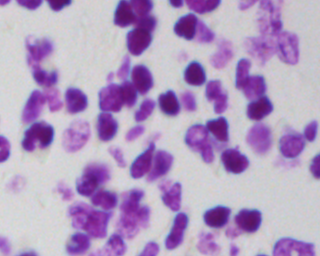
\includegraphics[width=.8\linewidth]{images/example_1.png}
  \caption{Obraz kolorowy}
  \label{fig:sub1}
\end{subfigure}%
\begin{subfigure}{.5\textwidth}
  \centering
  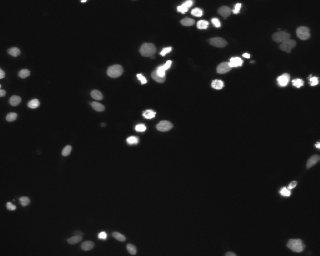
\includegraphics[width=.8\linewidth]{images/example_2.png}
  \caption{Obraz w odcieniach szarości}
  \label{fig:sub2}
\end{subfigure}
\caption{Przykładowe obrazy ze zbioru treningowego.}
\label{fig:examp1}
\end{figure}
\newline
Na Rysunku \ref{fig:examp2}. zostały zaprezentowane dwa obrazy. Pierwszy z nich przedstawia oryginalny obraz ze zbioru, natomiast drugi z nich przedstawia jedną, wybraną losowo maskę. Maska reprezentuje jedną wysegmentowaną komórkę z obrazu oryginalnego. W przypadku przedstawionego obrazu, w zestawie znajdują się 62~maski dla tego obrazu. 
\newline
\begin{figure}[h!]
\centering
\begin{subfigure}{.5\textwidth}
  \centering
  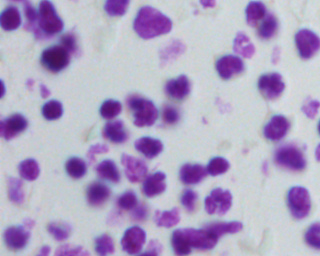
\includegraphics[width=.8\linewidth]{images/example_3.png}
  \caption{Obraz oryginalny}
  \label{fig:sub3}
\end{subfigure}%
\begin{subfigure}{.5\textwidth}
  \centering
  
\includegraphics[width=.8\linewidth]{images/example_3_mask.png}
  \caption{Wybrana maska}
  \label{fig:sub4}
\end{subfigure}
\caption{Przykładowy obraz oryginalnego obrazu oraz wybranej maski ze~zbioru treningowego.}
\label{fig:examp2}
\end{figure}
\newpage
\section{Możliwości programu}
\subsection{Cyfrowe przetwarzanie obrazów}
Korzystanie z programu będzie możliwe na dwa sposoby, które zostały wstępnie omówione w sekcji \textit{Opis problemu}. Pierwszą z tych metod będzie cyfrowe przetwarzanie obrazów. Jest to bardzo dobrze rozwinięta dyscyplina, która pozwala modyfikować obrazy na poziomie pojedynczych pikseli. W szczególności zostaną wykorzystane elementy morfologii matematycznej. Program działający w tym trybie będzie potrzebował jedynie ścieżki do pliku, która będzie podawana jako argument uruchomienia programu.
\subsection{Sieci neuronowe}
Kolejnym sposobem korzystania z programu będzie wyorzystanie sztucznej sieci neuronowej. W tym przypadku program będzie mógł działać w dwóch trybach. Pierwszy z nich będzie służył do zliczania komórek, podobnie jak w przypadku cyfrowego przetwarzania obrazów. Drugi tryb będzie niezbędny do wytrenowania modelu, który jest nieodzownym elementem tej dziedziny. Dzięki temu program będzie miał dodatkową funkcjonalność, która pozwoli w pełni dostosować program do indywidualnych potrzeb, poprzez wytrenowanie sieci neuronowej na~własnym zbiorze danych zawierającym obrazy oryginalne oraz maski do każdego z nich.
\section{Użytkowanie programu}
\subsection{Typ programu}
Program zostanie zaimplementowany w języku \textit{Python}, natomiast będzie on uruchamiany z poziomu wiersza poleceń. Dodatkowo program będzie przenośny między popularnymi systemami operacyjnymi, pochodzącymi z rodziny \textit{Linux/Unix} oraz systemami z rodziny \textit{Microsoft Windows}.
\subsection{Oczekiwany rezultat}
W przypadku, zliczania komórek na obrazie, program wypisze na ekran następującą treść:
\begin{verbatim}    The image contains 32 cells.\end{verbatim}
gdzie 32 jest przykładową liczbą.
\newline
\newline
Program dodatkowo może wyświetlać poszczególne etapy realizacji procesu zliczania komórek, bądź procesu uczenia sieci neuronowej, w celu poinformowania użytkownika o dotychczsowym stanie programu.
\subsection{Uruchomienie programu}
Poniżej zostanie przedstawione przykładowe uruchomienie programu z uwzględnieniem systemu operacyjnego. W przypadku systemu operacyjnego z rodziny \textit{Linux/Unix} program należy uruchomić w następujący sposób:
\begin{verbatim}
    python3 biological_cells_counter.py -file path_to_file
\end{verbatim}
Natomiast w przypadku systemu operacyjnego z rodziny \textit{Microsoft Windows} będzie to wyglądało następująco:
\begin{verbatim}
    python biological_cells_counter.py -file path_to_file
\end{verbatim}
Zarówno w pierwszym, jak i drugim przypadku, podczas zliczania komórek, niezbędna jest ścieżka do pliku, bez której program zakończy swoje działanie bez wykonania głównego zadania. Domyślnie program będzie zliczał komórki z~wykorzystaniem algorytmu zaimplementowanego w oparciu o cyforwe przetwarzanie obrazów.
\subsection{Parametry programu}
W celu wykorzystania wszystkich możliwości dostarczonych do programu należy używać flag zgodnie z ich przeznaczeniem, w sposób zademonstrowany w sekcji \textit{Uruchomienie programu}. W programie będziemy mogli użyć następujących flag:
\begin{itemize}
    \item -file -- za pomocą tej flagi wskazywany jest plik z obrazem zawierającym komórki do zliczenia,
    \item -output -- za pomocą tej opcjonalnej flagi wskazywana jest ścieżka i plik do którego ma zostać zapisany obraz z wysegmentowanymi komórkami,
    \item -mode -- za pomocą tej flagi ustawiany jest tryb, w którym będą zliczane komórki, użytkownik jako argument może podać następujące wartości:
    \begin{itemize}
        \item dip -- [domyślne ustawienie] skrót od nazwy \textit{cyfrowe przetwarzanie obrazów} (\textit{ang. digital image processing}),
        \item nn -- skrót od nazwy \textit{sieć neuronowa} (\textit{ang. neural network}),
        \item tnn -- skrót od nazwy \textit{trenowanie sieci neuronowej} (\textit{ang. training neural network}),
    \end{itemize}
    \item -params -- za pomocą tej flagi przekazywane są niezbędne parametry do~uczenia sieci, takie jak liczba epok, katalog z obrazami oryginalnymi czy~katalog z maskami. Należy pamiętać, aby argumenty zostały przekazane w~cudzysłowie, argument ten jest wymagany w przypadku, gdy flaga \textit{mode} przyjmuje wartość \textit{tnn}.
    \item -h lub --help -- za pomocą tych flag, użytkownik będzie miał możliwość wyświetlenia opcji oraz ich krótkich opisów, które są dostępne w programie.
\end{itemize}
\subsection{Obsługa błędów}
Program będzie w stanie obsłużyć podstawowe błędy, które mogą powstać w~przypadku błędnego korzystania z programu przez użytkownika. Poniżej zostaną przedstawione obsługiwane przez program błędy:
\begin{enumerate}
    \item Brak niezbędnego argumentu.
    \newline
    W przypadku braku niezbędnego argumentu, program poinformuje użytkownika za pomocą wypisania na ekran następującej informacji:
    \begin{verbatim}    Missing argument: argument\end{verbatim}
    Jako brakujący argument można przyjąć niezdefiniowanie argumentu \textit{parms}, gdy program ma pracować w trybie uczącym [\textit{-mode tnn}] lub brak argumentu [\textit{-file path\_to\_file}], gdy program ma zliczać komórki na obrazie.
    \item Niepoprawna flaga.
    \newline
    W przypadku, gdy użytkownik poda niepoprawną (niezdefiniowaną) flagę, program poinformuje użytkownika za pomocą wypisania na ekran następującej informacji:
    \begin{verbatim}    Unrecognized arguments: argument\end{verbatim}
    Taka sytuacja może mieć miejsce, gdy użytkownik użyje flagi [\textit{-f file\_to\_path}], zamiast flagi [\textit{-file file\_to\_path}].
    \item Niepoprawny tryb.
    \newline
    W przypadku, gdy użytkownik poda niepoprawny tryb, program poinformuje użytkownika za pomocą wypisania na ekran następującej informacji:
    \begin{verbatim}    Unrecognized mode: argument\end{verbatim}
    Możliwe jest tylko wykorzystanie zdefiniowanych trybów, które zostały opisane powyżej [\textit{dip, nn, tnn}]. Użycie każdego innego trybu doprawdzi do wystąpienia błędu.
    \item Niepoprawna ścieżka do pliku
    \newline
    W przypadku, gdy użytkownik poda niepoprawną ścieżkę do pliku, program poinformuje użytkownika za pomocą wypisania na ekran następującej informacji:
    \begin{verbatim}    File not found: path_to_file\end{verbatim}
    \newpage
    \item Niepoprawne argumenty do uczenia sieci neuronowej.
    \newline
    W przypadku, gdy użytkownik poda niepoprawne argumenty służące do~procesu trenowania sieci neuronowej, program poinformuje użytkownika za~pomocą wypisania na ekran następującej informacji:
    \begin{verbatim}    Incorrect arguments to learning: arguments\end{verbatim}
    \item Zbyt dużo argumentów.
    \newline
    W przypadku, gdy użytkownik poda zbyt dużą liczbę argumentów, program będzie dopasowywał argumenty do trybu w którym pracuje, a nadmiarowe argumenty nie zostaną wykorzystane.
\end{enumerate}

\label{end}
\end{document}